\documentclass[a4paper,10pt]{article}
\usepackage[utf8]{inputenc}
\usepackage{geometry}
\usepackage{graphicx}
\geometry{margin=1in}

\usepackage{xcolor}
\usepackage{hyperref}
\hypersetup{colorlinks=true,linkcolor=blue,urlcolor=blue}
\urlstyle{rm}

\usepackage{attachfile2} % for attaching files to the rendered PDF: \attachfile{example.xlsx}

\usepackage{embedfile}
\usepackage{hypgotoe}
\embedfile{references/resume-references.pdf}
\embedfile{references/42Transcript.pdf}


\usepackage{array}

%------------------------------------------------

\begin{document}

\title{Attila NÉMET}
% \author{Attila Német}
\date{}
\maketitle


% \hspace{-0.5cm}
\begin{minipage}[t]{0.14\textwidth}
    \vspace{0pt} % Aligns the top of the image with the text
    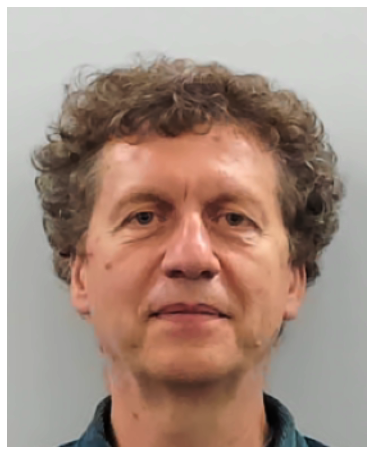
\includegraphics[width=\textwidth]{img/myself_ID.png} % path to the image
\end{minipage}
\hfill
% \hspace{0.1\textwidth}
\begin{minipage}[t]{0.66\textwidth}
    \vspace{0pt} % Aligns the top of the image with the text
    \subsection*{Contact Information}
    \begin{tabbing}
        \hspace{2.55cm} \= \hspace{3cm} \= \kill % Set tab stops
        \textbf{Mobile}:  \> +352-661-118922 \\
        \textbf{Email}:  \> \href{mailto:attila.nemet@gmail.com}{attila.nemet@gmail.com} \\
        \textbf{LinkedIn}:   \> \href{https://www.linkedin.com/in/attilanemet}{https://www.linkedin.com/in/attilanemet} \\
        \textbf{Address}:   \> 29 rue Jean-Pierre Sauvage, 2514 Luxembourg \\
    \end{tabbing}
    \end{minipage}

\subsection*{Summary}
Senior telecom and software engineering professional with 20+ years of international experience at Ericsson, including technical lead responsibilities, backend-oriented automation, large-scale network configuration, testing, and database-backed rollout activities. Strong Python and scripting background, deep domain knowledge in telecommunications, and proven delivery in complex multi-country projects.

Recent academic and hands-on work further strengthened my software engineering profile through AI/ML projects, LLM-based software testing research, and the 42 Luxembourg curriculum in C/C++, Unix, networking, web, and systems programming. I am targeting senior software engineering roles where my technical leadership, telecom expertise, backend mindset, and modern software upskilling can contribute to cloud and full-stack product development.

\subsection*{Education}
\begin{itemize}
    \item \textbf{Present}: 42 School, Luxembourg\\
    \href{gotoe:embedded=references/42Transcript.pdf}{Project-based learning}, currently at level 9.70 with 87\% of the common core completed; hands-on work in C, C++, Unix, networking, systems programming, graphics, and web fundamentals
    \item \textbf{September 2024}: University of Luxembourg\\
    Master in Space Technologies and Business
    \item \textbf{June 1991}: Technical University of Cluj-Napoca, Romania\\
    Electronics \& Telecommunication
\end{itemize}

\subsection*{Relevant Skills and Experiences}
\begin{itemize}
    \item \textbf{Technical Leadership \& Delivery:} Led and supported complex telecom modernization and rollout projects across 20+ countries, coordinating implementation, procedures, tooling, and execution in live environments.
    \item \textbf{Backend Automation \& Scripting:} Proficiency in Python and Perl for configuration generation, process automation, rollout support, and data handling in telecom and network engineering contexts.
    \item \textbf{Telecommunications Domain Expertise:} Extensive experience across mobile and fixed networks, including 2G/3G/4G/5G, RAN, RNC, MSS, IN, deployment, integration, support, load testing, and network modernization.
    \item \textbf{Software Testing using LLMs:} Studied the possibility to use LLMs for testing of space software and wrote my
    \href{https://gitlab.com/uniluxembourg/snt/svv/msc/nemet-attila-istvan-msc/thesis_work/-/blob/main/A.Nemet_Thesis_TMT__LLM.pdf}{ master thesis}
    in this subject.
    \item \textbf{Scientific Space Project:} Generation of Training Images for Lens Flare Removal -- developing the LFW (\href{https://github.com/dajcs/LFW}{Lens Flare Wizard}), a Python and Blender-based toolkit for augmenting training datasets with realistic lens flare effects to train computer vision models against lens flare artifacts.
    \item \textbf{AI \& Machine Learning:} Developed a concept for mass configuration of telecom equipment using ML/AI and complemented it with extensive self-study and graduate-level project work.
    \item \textbf{Systems, Networking \& Web Foundations:} Built strong low-level software foundations at 42 Luxembourg, including sockets, processes, Linux/Unix, concurrency, graphics, and web fundamentals relevant to backend and full-stack engineering.
    \item \textbf{Databases \& Data Handling:} Managed and used operational databases in rollout and modernization activities; comfortable working with structured data, XML, JSON, and Python data tooling.
    \item \textbf{Teamwork \& Communication:} Worked in 20+ countries
    (\href{gotoe:embedded=references/resume-references.pdf}{resume-references.pdf}).
    Collaborated with diverse teams across different projects. Provided support and effectively communicated with POs (Product Owners).
\end{itemize}
% icon =  Paperclip | PushPin | Graph | Tag

\subsection*{Languages}
\begin{tabbing}
    \hspace{0.55cm} \= \hspace{2.55cm} \= \hspace{3cm} \= \kill % Set tab stops
    \> \textbf{English}:  \> C2 -- Fluent \\
    \> \textbf{Romanian}:  \> C2 -- Fluent \\
    \> \textbf{French}:   \> B2 -- Intermediate \\
    \> \textbf{German}:   \> B1 -- Intermediate \\
    \> \textbf{Hungarian}: \> L1 -- Mother tongue \\
\end{tabbing}


\subsection*{Technical Strengths}
% \begin{tabular}{@{} >{\bfseries}l @{\hspace{6ex}} l @{}}
%     Computer Languages & C, Perl, Latex, Python, AI/ML, LLM \\
%     Protocols \& APIs & XML, JSON, numpy, pandas, matplotlib \\
%     % Databases & PostgreSQL \\
%     Tools & Visual Studio Code, Jupyter Notebook, Git
% \end{tabular}

\begin{tabbing}
    \hspace{0.55cm} \= \hspace{4.55cm} \= \hspace{3cm} \= \kill % Set tab stops

    \> \textbf{Languages}:  \> Python, C, C++, Perl, JavaScript fundamentals, LaTeX \\
    \> \textbf{Backend / Data}:  \> XML, JSON, numpy, pandas, matplotlib, scripting, automation \\
    \> \textbf{Systems / Web}:   \> Unix/Linux, sockets, processes, networking, HTTP, web fundamentals \\
    \> \textbf{Tools}:   \> Git, Visual Studio Code, Jupyter Notebook, Blender \\
    \> \textbf{AI / LLM}:   \> MS Copilot, Claude Code, MCP, Skills, LangChain \\

\end{tabbing}



\subsection*{Selected Work Experiences with Ericsson}
\begin{itemize}
    \item \textbf{Apr 2015 -- Apr 2023, Budapest}: Business Analyst / Software Tester
    \begin{itemize}
        \item Worked on mass configuration concepts for telecom equipment using AI and ML.
        \item Designed and performed load tests on routers and 4G/5G telecom nodes.
        \item Contributed to software quality, large-scale configuration validation, and backend-oriented test preparation.
    \end{itemize}
    \item \textbf{Nov 2014 -- Mar 2015, Budapest}: Consultant
    \begin{itemize}
        \item Advised on the development of a configuration tool for RAN telecom nodes.
    \end{itemize}
    \item \textbf{Jul 2014 -- Oct 2014, Budapest}: Network Optimization Engineer
    \begin{itemize}
        \item Implemented and developed scripts for Irish operator networks to improve RAN performance.
    \end{itemize}
    \item \textbf{May 2013 -- Jun 2014, Dublin}: 4G Rollout, RAN modernization Technical Lead
    \begin{itemize}
        \item Led development and implementation of scripts, procedures, and databases for O2 and Meteor 4G rollout activities.
        \item Developed scripts and procedures for Vodafone Ireland 3G RBS rehoming.
        \item Combined technical leadership, delivery coordination, automation, and operational rigor in a live telecom environment.
    \end{itemize}
    \item \textbf{Feb 2011 -- Dec 2012, Düsseldorf}: Integration \& Configuration \& Procedure Development
    \begin{itemize}
        \item Developed and executed RNC data conversion and modernization swap procedures for live networks.
        \item Delivered a successful rollout approach despite developing the procedure without access to test nodes.
    \end{itemize}
    \item \textbf{Feb 2010 -- Feb 2011, Dublin}: Network Integration and Automation Engineer
    \begin{itemize}
        \item Performed RBS swap and integration in Vodafone, O2, and Meteor networks in Ireland.
        \item Wrote Perl scripts to generate RBS configuration files.
    \end{itemize}
\end{itemize}

\subsection*{Relevant AI/ML Online Courses}
\begin{itemize}
    \item \textbf{LLM Engineering:}
    \begin{itemize}
        \item Master AI, Large Language Models \& Agents
    \end{itemize}
    \item \textbf{Andrej Karpathy's Tutorials}:
    \begin{itemize}
        \item GPT Tokenizer
        \item Reproducing GPT-2
    \end{itemize}
    \item \textbf{Udacity}:
    \begin{itemize}
        \item Self-Driving Car Nanodegree (T1)
        \item Machine Learning Engineer Nanodegree
        \item Deep Learning Foundations Nanodegree
    \end{itemize}
    \item \textbf{Coursera}:
    \begin{itemize}
        \item Machine Learning (Stanford University)
        \item Using Databases with Python (University of Michigan)
        \item State-Estimation and Localization for Self-Driving Cars (University of Toronto)
    \end{itemize}
\end{itemize}

\subsection*{References}
\begin{tabbing}
    \hspace{0.55cm} \= \hspace{4.55cm} \= \hspace{3cm} \= \kill % Set tab stops

    % \> \href{https://www.linkedin.com/in/carolroboticvision/}{\textbf{Carol Martinez}}  \> RMS (Robotic Manipulation in Space) professor\\
    \> \href{https://www.linkedin.com/in/jorgequerol/}{\textbf{Jorge Querol}}  \> SatCom (Satellite Communications) professor\\
    % \> \href{https://www.linkedin.com/in/raonilourenco/}{\textbf{Raoni Lourenço}}  \> ML (Machine Learning) teacher\\
    \> \href{https://www.linkedin.com/in/djamilaaouada/}{\textbf{Djamila Aouada}}  \> CVIA (Computer Vision and Image Analysis) professor\\
    \> \href{https://www.linkedin.com/in/fabrizio-pastore-41226b4/}{\textbf{Fabrizio Pastore}}  \> Space Informatics professor, Master Thesis supervisor\\
    \> \href{https://www.linkedin.com/in/miguel-a-olivares-mendez-8a952533/}{\textbf{Miguel Olivares-Mendez}}  \> Space Robotics professor, Scientific Project supervisor\\
    % \> \href{https://www.linkedin.com/in/holger-voos-85864938/}{\textbf{Holger Voos}}  \> GNCSS (Guidance, Navigation and Control for Space Systems) professor\\
    \> \href{https://www.linkedin.com/in/christian-fisch-7745ba167/}{\textbf{Christian Fisch}}  \> Business Economics and Entrepreneurship professor\\

\end{tabbing}


\end{document}
